
\section{Design}
\label{sec:design}
In this section, we present the two-tier compiler-serving co-design of \sysname. As shown in Figure~\ref{fig:design_overview}, \emph{agent descriptor} is generated by the combination of analyzing agent program and observing runtime behaviors. Server side then exploits the derived descriptor to schedule the KV-cache efficiently, using \emph{adaptive prompt re-layout} (\S\ref{sec:relayout}) and \emph{proactive KV-cache scheduling} (\S\ref{sec:Proactive KV-Cache Scheduling}).

\begin{figure}[h]
    \centering
    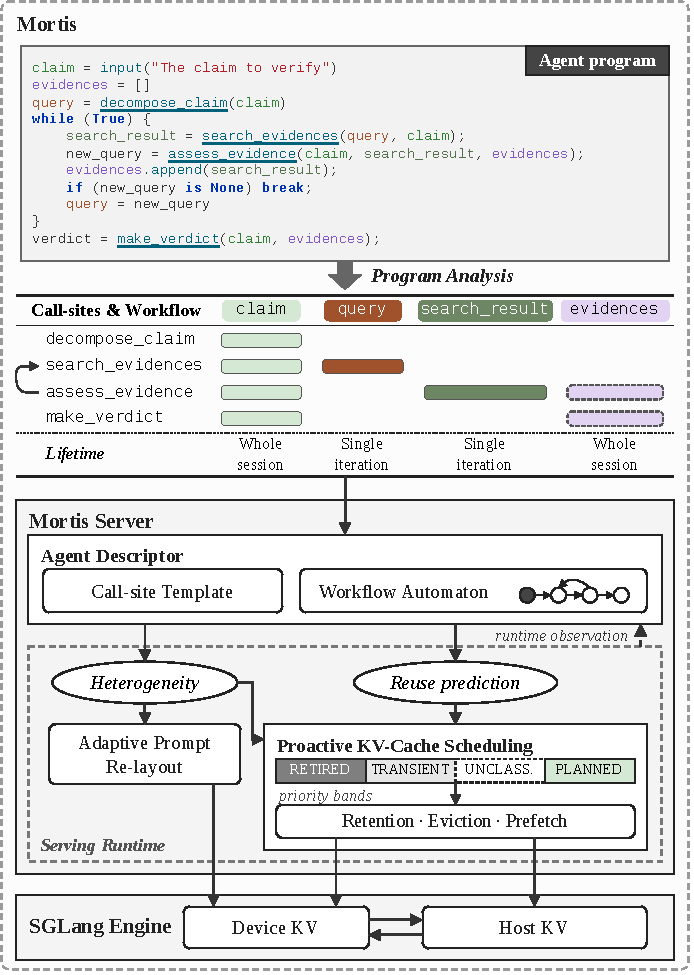
\includegraphics[width=0.95\columnwidth]{ArchOverview.pdf}
    \caption{Architecture overview of \sysname.}
    \label{fig:design_overview}
\end{figure}


\subsection{Agent Descriptor}
\emph{Agent descritor} contains the metadata for scheduling. Static analysis provides it a skeleton and the server refines the weights with runtime observations. An agent descriptor contains two parts: 
\begin{enumerate*}[label=(\roman*)]
    \item \textbf{Call-site Template:} It provides a heuristic of the components' lifetime, sharing scope and evolution pattern.
    \item \textbf{Workflow Automaton:} It contains the program-level structure of an agent, including workflow dependencies, execution time estimation and transition probabilities.
\end{enumerate*} 

\sysname traverses the agents type-checked AST to identify LLM call sites and their relationships. It then classifies each parameter's provenance and lifetime to construct the skeleton of the agent descriptor.
\subsubsection{Call-site Template}
\label{sec:template}
As discussed in \S\ref{sec:motivation}, the components of a programmatically generated prompt can be classified into the following two categories:
\begin{enumerate*}[label=(\roman*)]
    \item \textbf{Invariant Specifications:} the components that are fixed once the program is compiled, such as the system prompt, response schema, and the tool declarations. They are rendered from the compiler's own intermediate representation and stay constant.
    \item \textbf{Dynamic Bindings:} because LLM calls are declared as ordinary functions, the arguments of a call site are supplied at runtime. These runtime values are the dynamic bindings.
\end{enumerate*}

We therefore define the call-site template as
\[
\mathcal{T}_c=\langle \mathcal{I}_c,\ \mathcal{B}_c,\ \mathcal{H}_c \rangle ,
\]
where $\mathcal{I}_c$ is the invariant specifications, $\mathcal{B}_c$ is the dynamic bindings, and $\mathcal{H}_c$ is the heterogeneity annotation over those bindings. All three are recovered by static analysis. 

\paragraph{Heterogeneity annotation.}
For each dynamic binding, $\mathcal{H}_c$ records both how its value is shared and how long that value stays valid:
\[
\mathcal{H}_c:\ \mathcal{B}_c \longrightarrow \mathcal{E} \times \mathcal{S} .
\]
The sharing pattern component $\mathcal{E}$ classifies a binding by its value provenance. We distinguish $\mathcal{E}$ into five classes, listed from the most to the least reusable:
\begin{enumerate*}[label=\textbf{(\roman*)}]
    \item \textbf{CONST:} the value is fixed by the program text and is identical at every call.
    \item \textbf{COPY:} the value is the same as the value another call site carries, so the bytes are already resident once that call site has run.
    \item \textbf{RESP:} the value comes from the reply produced by another call site.
    \item \textbf{EXTEND:} the binding is an append-only context, and the previous value remains a prefix of the new one.
    \item \textbf{VOLATILE:} the value is freshly produced at each call, or its origin lies outside what the analysis can see.
\end{enumerate*}
We write $\rho$ for the rank of a class in the order above, which expresses how much of a binding's bytes an earlier call can already supply. 

The lifetime component $\mathcal{S}$ names the program scope whose completion invalidates a binding's value ($\mathcal{S}=\emptyset$ meaning that the value survives for the whole session once produced). 

The evolution component $\mathcal{E}$ governs which bytes a later prompt can reuse, while the lifetime component $\mathcal{S}$ governs when cached bytes can be given up.

\subsubsection{Workflow Automaton}
\label{sec:TPFM}
An agent typically consists of a sequence of dependent LLM calls whose workflow structure is encoded in the program. Concretely, we abstract an agent as a time-annotated probabilistic finite-state machine (TPFM). We formulate the TPFM as: 
\[
\mathcal{A} = (Q, P, q_0, F, \mathcal{T}),
\]
where:
\begin{enumerate*}[label=(\roman*)]
    \item $Q$ is the set of states. Each state $q\in Q$ is labeled by an LLM callsite;
    \item $P$ denotes the transition probabilities between states.
    \item $q_0 \in Q$ is the entrance callsite.
    \item $F$ specifies the termination probability of the agent at each state.
    \item $\mathcal{T} = \left\{D^{\mathrm{exec}}_q, D^{\mathrm{gap}}_{q,q'}\right\}$ denotes the timing annotations associated with states and transitions, where $D^{\mathrm{exec}}_q$ is the execution-time distribution of the LLM callsite represented by state $q$, and $D^{\mathrm{gap}}_{q,q'}$ is the inter-call gap distribution between the completion of callsite $q$ and the invocation of its successor $q'$.
\end{enumerate*}

Static analysis fixes the shape of this automaton, while its weights come from runtime logs. The states, the entry, the transitions among them, and final states are recovered from code. $\mathcal{T} = \left\{D^{\mathrm{exec}}_q, D^{\mathrm{gap}}_{q,q'}\right\}$ and $P$ are often unknown at compile time and model-dependent. The server observes these online and accumulates them across sessions, updating the statistical model of the agent consistently. Together the two halves give the server a forward-looking view of a session.

\subsection{Adaptive Prompt Re-layout}
\label{sec:relayout}
Prefix reuse stops at the first byte that differs from a cached prompt. The message a framework emits for a call site follows the declaration order of the function, which may place a changing value ahead of values that later calls could reuse. \sysname's adaptive re-layout permutes the components of each call message so that the bytes most likely to be resident already come first. The descriptor $\mathcal{T}_c$ (\S\ref{sec:template}) and $\mathcal{A}$ (\S\ref{sec:TPFM}) determine a partial order over the components, and the server completes it into a layout with the token lengths it observes at runtime.
\subsubsection{Movable Components}
First, the dynamic bindings $\mathcal{B}_c$ can be permuted freely. The compiler lowers each argument into a self-contained component labeled by its parameter name, and the framework places these components in declaration order only because that is the order of the argument list; re-layout may therefore choose any order of the bindings.

Second, part of the invariant specification $\mathcal{I}_c$ is movable as well. $\mathcal{I}_c$ is treated as one block abstraction in \S\ref{sec:template}, but it has internal structure. It consists of the system prompt, the response schema, the tool schema, and the instruction specification (the task description and parameter descriptions generated by the compiler). Among them, the system prompt stays universally constant, and the two schemas are consumed by the model separately. The instruction specification is movable. 

\sysname therefore operates on the order of bindings and the placement of instruction specification. \S\ref{sec:layout_decision} describes how \sysname chooses a layout within this space.

\subsubsection{Layout Decision}
\label{sec:layout_decision}
Each call site sorts the bindings it carries by a program-wide key. Generally, \emph{shared} bindings, which are carried by multiple call sites, are placed at the front, followed by the bindings carried by a single call site. Algorithm~\ref{alg:layout} summarizes the procedure.

\paragraph{Sorting private bindings.} The bindings carried by a single call site are sorted in ascending lexicographic order of
\[
K(b)=\big(\textit{scoped},\ \rho,\ \textit{depth},\ -\textit{length}\big),
\]
whose components are defined as follows:
\begin{enumerate*}[label=\textbf{(\roman*)}]
    \item \textit{scoped}: the lifetime of $b$; 0 if it is session-wide ($\mathcal{S}=\emptyset$) and 1 otherwise, so bindings that survive scope boundaries precede those reset by them.
    \item $\rho$: the stability rank defined in \S\ref{sec:template}, from 1 for CONST to 5 for VOLATILE, so the more reusable class leads.
    \item \textit{depth}: The number of transitions to the first call site that carries it from entrance, so values that enter a session earlier lead.
    \item \textit{length}: the token length of the value of $b$, observed by the server; negated so longer bindings precede.
\end{enumerate*}

\paragraph{Sorting shared bindings.} The order of shared bindings is derived from program-level structures. For every transition from $q$ to $q'$, \staticAnalysis identifies how each shared binding of the two call sites evolves. We categorize these patterns into three groups, ordered as follows:
\begin{enumerate*}[label=(\textbf{\roman*})]
    \item Both call sites carry it and its value does not change between the two calls.
    \item Both call sites carry it and the program only appends to its value.
    \item Program rewrites it between the two calls, or only one of the two call sites carries it.
\end{enumerate*}

\sysname collects these requirements over all transitions and orders the shared bindings to satisfy them; when several bindings can go next, the one with the smallest $\textbf{(-\textit{length}, \textit{depth})}$ is placed first. Bindings with conflicting requirements are clustered and sorted by the same key.

\paragraph{Placing the specification.} The \emph{instruction specification} is lowered from code by the compiler and is unique to each call site. Emitting it first would prevent prefix sharing among different call sites. After sorting, \sysname moves the specification to the end when the leading bindings are shared, so that sibling call sites can share larger common prefix. A switch keeps the specification in front when moving it is suspected of changing the model's behavior.

\begin{algorithm}[t]
\caption{Layout decision algorithm}
\label{alg:layout}
\begin{algorithmic}[1]
\algtext*{EndFor}\algtext*{EndIf}
\Require Descriptor $(\{\mathcal{T}_c\}_{c\in C},\mathcal{A})$, lengths $\ell$, switch $\textit{pin}$
\Ensure Layouts $\{L_c\}_{c\in C}$
\State $B_{\mathrm{sh}} \gets \{b : |\{c\in C : b\in\mathcal{B}_c\}| > 1\}$;\ \ $R \gets \emptyset$
\ForAll{$e=(q,q')\in\Call{Edges}{\mathcal{A}}$}
  \State $B_e \gets B_{\mathrm{sh}}\cap(\mathcal{B}_q\cup\mathcal{B}_{q'})$
  \State $t_e(b) \gets 1$ if \textit{unchanged}, $2$ if \textit{append-only}, else $3$
  \State $R \gets R\cup\{(b,b')\in B_e^2 : t_e(b)<t_e(b')\}$
\EndFor
\State $J(b) \gets (-\ell(b),\textit{depth}(b))$;\ \ $J_{\min}(S) \gets \min_{b\in S}J(b)$
\State $D \gets \Call{ClusterConflicts}{B_{\mathrm{sh}},R}$
\State $\langle S_1,\dots,S_k\rangle \gets \Call{TopoSort}{D,J_{\min}}$ \Comment{Min-key first}
\State $\pi_{\mathrm{sh}} \gets \Call{Sort}{S_1,J}\Vert\cdots\Vert\Call{Sort}{S_k,J}$
\ForAll{$c\in C$}
  \State $\pi_c \gets \langle b\in\pi_{\mathrm{sh}} : b\in\mathcal{B}_c\rangle\Vert\Call{Sort}{\mathcal{B}_c\setminus B_{\mathrm{sh}},K}$
  \State $s_c \gets \Call{InstructionSpec}{\mathcal{I}_c}$
  \State $L_c \gets \langle s_c\rangle \Vert \pi_c$
  \If{$\neg\,\textit{pin}\land(\mathcal{B}_c\cap B_{\mathrm{sh}}\ne\emptyset)$} $L_c \gets \pi_c \Vert \langle s_c\rangle$
  \EndIf
\EndFor
\State \Return $\{L_c\}_{c\in C}$
\end{algorithmic}
\end{algorithm}


\subsection{Proactive KV-Cache Scheduling}
\label{sec:Proactive KV-Cache Scheduling}
While adaptive prompt re-layout improves prefix reuse only by reshaping the request, \sysname's KV-cache scheduling proactively arranges the placement of KV-cache entries. Using the agent descriptor, the server decides for every served KV-cache sequence what to keep, what to give up, and what to prefetch.

\subsubsection{Reusable Head and Volatile Tail}
\label{sec:identify_reusable_kv}
Since re-layout already places the stable and shared bindings at the front, a served prompt naturally divides into two segments: a reusable head and a volatile tail. 

The reusable head consists of two parts: a \emph{static prefix} and a \emph{session-shared extension}:
\begin{enumerate*}[label=(\roman*)]
    \item \textbf{Static Prefix} is what the call site emits without runtime inputs, and its value outlives a single session. It includes the invariant specifications $\mathcal{I}_c$ together with the CONST bindings that re-layout has placed right behind $\mathcal{I}_c$.
    \item \textbf{Session-shared Extension} is the bindings behind the static prefix that a later call of the same session will emit again identically.
\end{enumerate*}
\sysname determine the reusable head by analyzing $\mathcal{H}_c$, $\mathcal{A}$ and the decided prompt layout jointly.

\subsubsection{Next-Call Prediction}
Our prediction focuses on the following three aspects:
\begin{enumerate*}[label=(\roman*)]
    \item The probability of the arrival.
    \item When the call will arrive.
    \item Which prefix of its prompt can be speculatively constructed.
\end{enumerate*}

\paragraph{Arrival probability.}
We estimate the probability of the next call by a loop-tagged table. \sysname adopts Bourdoncle-style~\cite{bourdoncle1993efficient} weak topological ordering to discover all loops within the agent based on the emitted workflow graph. Each call-site $q$ can be located by a chain of loops enclosing it; for each call-site's invocation, the server marks it with a tuple $\zeta=\left\{i_1, i_2, \dots, i_n\right\}$, where $i_k$ is the current iteration index of the $k$-th enclosing loop, outermost first. We define the table as:
\[
\mathcal{P}(q' \mid q, \zeta) \qquad \mathcal{F}(q, \zeta)
\]
Where $\mathcal{P}$ stands for the probability that a call-site $q$ in context $\zeta$ is followed by a call-site $q'$; $\mathcal{F}$ stands for the probability that the session ends at call-site $q$ under context $\zeta$. With an empty $\zeta$ (no loop context), $\mathcal{P}$ and $\mathcal{F}$ coincide with $P$ and $F$.

The table is a frequency count that the server updates across sessions. 
Let $q$ and $\zeta$ denote the call-site and loop context of the preceding call in the same session. When a call at $q'$ arrives, the server increments the count of outcome $q'$ in row $(q,\zeta)$; when the session closes at $q$, it increment termination count in also in row $(q,\zeta)$; Each observation is also counted in the row of every suffix of $\zeta$, down to the empty tuple, so that for the same $q$ the table holds one row per level of context. After a call at $q$ lands, we compute the probability of each outcome $o$ by Witten--Bell interpolation from the empty context $\zeta_0$ to the full context $\zeta_m=\zeta$, where $o$ ranges over $\mathrm{succ}(q)$, the static successors of $q$ plus a virtual outcome $\mathrm{end}$ for session termination:
\begin{align*}
\hat{P}_k(o) &= \lambda_k\,\frac{c_k(o)}{n_k}+(1-\lambda_k)\,\hat{P}_{k-1}(o),\qquad k=0,\dots,m, \\
\hat{P}_{-1}(o) &= \frac{1}{|\mathrm{succ}(q)|},\qquad
\lambda_k=\begin{cases}\dfrac{n_k}{n_k+d_k} & n_k>0,\\[4pt] 0 & n_k=0,\end{cases}
\end{align*}
where $\zeta_k$ is the suffix of $\zeta$ that keeps only the innermost $k$ indices, and the three counts are read from the row $(q,\zeta_k)$ of the table: $c_k(o)$ is how many times outcome $o$ followed a call at $q$ in context $\zeta_k$, $n_k=\sum_o c_k(o)$ is the number of observations in that row, and $d_k$ is the number of distinct outcomes with $c_k(o)>0$.

Then,
\[
\mathcal{P}(q'\mid q,\zeta)=\hat{P}_m(q') \qquad \mathcal{F}(q,\zeta)=\hat{P}_m(\mathrm{end})
\]
A level with no observation is skipped. The weight $\lambda_k$ grows with the support of a level, so a well-observed iteration dominates the prediction while a sparse one defers to the pooled behavior of $q$.

\paragraph{Arrival time.}
The time of arrival is conservatively approximated based on recorded statistics. The workflow automaton records $D^{\mathrm{gap}}_{q,q'}$ per transition: each time a call at $q'$ arrives, the server appends the interval between the reply of the preceding call at $q$ and this arrival. The interval is the agent's own time spent in its code between two calls. 

We estimate the gap before the next call as:
\[
\hat{g}= t_{50}-\tfrac{1}{2}(t_{90}-t_{50})
\]
where $t_{50}$ and $t_{90}$ are the 50th and 90th percentiles of the gap samples on the transition $(q,q')$; the predicted call is then expected $\hat{g}$ after the reply of the current call. The second term ensures that a transition with a more dispersed gap distribution receives a tighter estimate. 

\paragraph{Prefix reconstruction.}
As indicated in \S\ref{sec:identify_reusable_kv}, the prompt of the known successor $q'$ is reconstructible, or at least partially reconstructible. \sysname builds its prompt in the layout $L_{q'}$, using the values that the session already carries. The construction processes bindings in the order of $L_{q'}$ while consulting their evolution class, deducing values accordingly. The construction stops at the first binding with no known origin. Then the matched prefix is sent to the kv-planner for speculative preparation. 

\subsubsection{Lifecycle Bands}
As we discussed in \S\ref{sec:motivation}, different components have different lifetimes, sharing scopes, and evolution patterns. Therefore, relying on recency-based LRU would lead to suboptimal performance. \sysname adopts a banded priority and steers KV-cache eviction with it. 

\paragraph{Bands.}
We categorize KV-cache entries into four bands, from first evicted to last:
\begin{enumerate*}[label=(\arabic*)]
    \item \textbf{RETIRED:} the volatile tails of prompts belonging to completed sessions. 
    \item \textbf{TRANSIENT:} the volatile tail of a served prompt of a live session. The session that produced them will not present them again.
    \item \textbf{UNCLASSIFIED:} entries that analysis cannot categorize, such as the prompts of a program that was never registered. They keep the engine's default treatment.
    \item \textbf{PLANNED:} prefixes that a predicted call will reuse. Inside this band entries are ordered by the expected value of keeping them resident, defined next.
\end{enumerate*}

Eviction empties the lowest band first and falls back to recency only within a band, so KV-cache that will likely be reused leaves memory later. On the host tier it keeps LRU eviction except that retired segments go first, so a head the device gave up under pressure remains reloadable while it may still be needed. Additionally, KV-cache entries marked as \emph{TRANSIENT} are not admitted into the host tier, as they wouldn't be reused.  

\paragraph{Band transitions.}
Bands are assigned at three moments of a session's lifecycle.
\begin{enumerate*}[label=(\arabic*)]
    \item \textbf{When a served prompt enters the cache}, \sysname splits it at its reusable head (\S\ref{sec:identify_reusable_kv}). The volatile tail and the reply generated after it become \emph{TRANSIENT}; the head stays \emph{UNCLASSIFIED} until the next prediction refresh finds a successor call that starts with it, which promotes it to \emph{PLANNED}.
    \item \textbf{When a later call arrives}, the transition it takes may rewrite bindings that earlier heads carried. Each affected head is cut back to the prefix that survives the rewrite, and the bytes past it are demoted to \emph{TRANSIENT}.
    \item \textbf{When the session ends}, the volatile tails of every prompt it served drop to \emph{RETIRED}. Their heads stay \emph{UNCLASSIFIED} and age out by recency, since other sessions of the same program may still share them.
\end{enumerate*}

These bands are mirrored directly into the radix tree's eviction order. The band is the primary key of the eviction heap and recency breaks ties.

\subsubsection{Retention and Prefetch}
Based on the prediction, the kv-planner of \sysname conducts protection. Its duty is to ensure that the required prefix resides on the device, or at least on the host. Each prediction is summarized into a tuple of reconstructed prefix, arrival probability and estimated deadline:
\[
\textit{Prediction}=\left(\pi_{q'},\ \mathcal{P}(q'\mid q,\zeta),\ t_{\mathrm{reply}}+\hat{g}\right)
\]
where $\pi_{q'}$ is the prefix reconstructed for $q'$ and $t_{\mathrm{reply}}$ is the time the current call replied. Predictions are refreshed at every call, and are dropped when the predicted calls arrive or expire. Protection acts on this tuple in two ways: \emph{Retention} keeps $\pi_{q'}$ from leaving the device, and \emph{prefetch} restores the part of $\pi_{q'}$ that has already been demoted to the host.

\paragraph{Retention.}
The planner ranks the predicted reusable KV-cache entries by the value of keeping $\pi_{q'}$ resident at every refresh:
\[
\mathcal{D}(q')=\frac{\mathcal{P}(q'\mid q,\zeta)\cdot |\pi_{q'}|_{\mathrm{cached}}}{\max\!\left(t_{\mathrm{reply}}+\hat{g}-t_{\mathrm{now}},\ \tau_{\min}\right)}
\]
where $|\pi_{q'}|_{\mathrm{cached}}$ is the number of tokens of $\pi_{q'}$ cached (on either host or device) and $\tau_{\min}$ is a floor that keeps a call due now from dominating. \sysname's kv-planner sorts all predictions by $\mathcal{D}$ in descending order, and admits them into \emph{PLANNED} until the band covers a fixed fraction of the device tier. Within the band, their $\mathcal{D}$ add up on every radix cache node, so that a shared head outranks a private one.

\paragraph{Prefetch.}
When part of $\pi_{q'}$ has been demoted to the host, the planner prefetches it back to the device ahead of the estimated arrival time. A prefetch release deadline is defined as: 
\[
t_{\mathrm{release}}=t_{\mathrm{reply}}+\hat{g}-\frac{|\pi_{q'}|_{\mathrm{host}}}{B_{\mathrm{h2d}}}-\frac{|\pi_{q'}|_{\mathrm{uncached}}}{B_{\mathrm{prefill}}}
\]
where $B_{\mathrm{h2d}}$ and $B_{\mathrm{prefill}}$ are the measured host-to-device copy rate and prefill rate. Among released predictions, the earliest deadline goes first, with ties broken by expected saving:
\[
\textit{Saving}=\mathcal{P}(q'\mid q,\zeta)\cdot|\pi_{q'}|_{\mathrm{cached}}
\]
A prefetch is released when the engine is idle or its deadline $t_{\mathrm{release}}$ approaches. It takes only free device memory, after reclaiming \emph{RETIRED} and \emph{TRANSIENT} entries. When no space is free, prefetching pauses but keeps touching its entries on the host so they do not age out by recency. 

